\documentclass[xcolor=dvipsnames]{beamer}

\mode<presentation> {

%Template by Crystal Nguyen
%12/4/2017

\usecolortheme{default}
%\setbeamercovered{transparent}

%\definecolor{carolina}{HTML}{82CAFA}
\definecolor{carolina}{HTML}{3BB9FF}
%\definecolor{gray}{HTML}{B6B6B4}
%\definecolor{dark}{HTML}{151B54}

\usetheme{Madrid}
\setbeamercolor{structure}{fg=carolina}
\setbeamercolor{block title}{bg=carolina}

%Uncomment the following if you prefer for the font color on carolina blue background to be black.
%\setbeamercolor{block title}{fg=black,bg=carolina}
%\setbeamercolor{frametitle}{fg=black}
%\setbeamercolor{title}{fg=black}

\setbeamertemplate{caption}[numbered]
\setbeamertemplate{enumerate items}[circle]
\setbeamertemplate{itemize items}[circle]
\setbeamertemplate{section in toc}[circle]
\setcounter{tocdepth}{1} 
\setbeamercolor{section in toc}{fg=black}

\usefonttheme[onlymath]{serif}

%\setbeamertemplate{footline} % To remove the footer line in all slides uncomment this line
%\setbeamertemplate{footline}[page number] 

% To replace the footer line in all slides with a simple slide count uncomment this line
%\setbeamertemplate{navigation symbols}{}

% To remove the navigation symbols from the bottom of all slides uncomment this line
}

%some commonly used packages
\usepackage{graphics}
\usepackage{graphicx}
\usepackage{tikz}
\usepackage{fancyvrb}
\usepackage{comment}
\usepackage{amsmath}
\usepackage{amssymb}
\usepackage{lipsum}
\usepackage{caption}
\usepackage{setspace}
\usepackage{tikz}
\usepackage{comment}
\usepackage{multirow}
\usepackage{float}

\newcommand{\overbar}[1]{\mkern 1.5mu\overline{\mkern-1.5mu#1\mkern-1.5mu}\mkern 1.5mu} %Instead of \bar or \overline, use \overbar for proper length and thickness bar for sample average. 


%To suppress numbering appendix slides
\newcommand{\backupbegin}{
	\newcounter{framenumberappendix}
	\setcounter{framenumberappendix}{\value{framenumber}}
}
\newcommand{\backupend}{
	\addtocounter{framenumberappendix}{-\value{framenumber}}
	\addtocounter{framenumber}{\value{framenumberappendix}} 
}

%For having footnote citations on slides
\usepackage{hanging}% http://ctan.org/pkg/hanging
\setbeamertemplate{footnote}{%
	\hangpara{2em}{1}%
	\makebox[2em][l]{\insertfootnotemark}\footnotesize\insertfootnotetext\par%
}

\newcommand\blfootnote[1]{%
	\begingroup
	\renewcommand\thefootnote{}\footnote[frame]{#1}%
	\addtocounter{footnote}{-1}%
	\endgroup
}
\setbeamerfont{footnote}{size=\tiny}

%Some macros
\DeclareMathOperator*{\argmin}{argmin} 
\DeclareMathOperator*{\argmax}{argmax}
\def\bs{\boldsymbol}
\def\l{\left}
\def\r{\right}     

\newcommand\Fontvi{\fontsize{8}{10}\selectfont}



%Edit the following lump of code to customize with your name, title, and date
\title[MS Presentation Template]{Title Slide Title}
\author[Last]{First Last}
\institute[UNC]{University of North Carolina at Chapel Hill}
\date{THE DATE}

\begin{document}
%example code of the title page
\begin{frame}
\titlepage
\begin{figure}
\begin{flushleft}

\includegraphics[scale=0.3]{unc_gillings_logo.png}
\end{flushleft}
\end{figure}
\end{frame}


\begin{frame}
\frametitle{Overview}
\tableofcontents
\end{frame}

\section{Background: Motivation}
\begin{frame}
\frametitle{Background}
\begin{itemize}
	\item Talk about your motivation
\end{itemize}
\end{frame}


%This example shows you how to:
%1. Use minipage to get multiple columns
%2. Use the \only command, so that it is the same numbered slide (slide 4), but when you hit next, you can change the color of the text
%3. USE VFILL. Vfill spaces out your bullets to take up the whole slide
\begin{frame}
\frametitle{Background: Motivation}
\begin{minipage}[t]{.3\textwidth}
	\begin{figure}[h!]
		\centering
		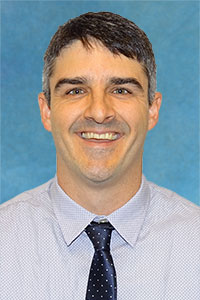
\includegraphics[height = 0.65\textwidth]{Corey.jpg}
		\caption*{Dr. Corey Kalbaugh}	
	\end{figure}
\end{minipage}\hfill 
\begin{minipage}[t]{.3\textwidth}
	\begin{figure}[h!]
		\centering
		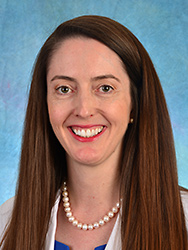
\includegraphics[height = 0.65\textwidth]{kibbe.jpg}
		\caption*{Dr. Melina Kibbe}
	\end{figure}
\end{minipage}\hfill
\begin{minipage}[t]{.3\textwidth}
	\begin{figure}[h!]
		\centering
		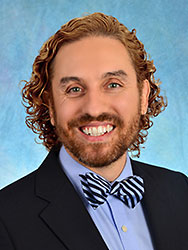
\includegraphics[height = 0.65\textwidth]{edward.jpeg}
		\caption*{Dr. Edward Bahnson}
	\end{figure}
\end{minipage}
\vfill
\begin{enumerate}
\item Scientific Study
\vfill
\item {\only<2>{\color{red}}Clinical Trial}
\vfill
\item {\only<2>{\color{red}}Observational Study}
\end{enumerate}
\end{frame}





%%%%%%%%%%%%%%%%%%%%%%%%%%%%%%%%%%%%%%%%%%%%%%%%%%%%%%%%%%%%%%%%%%%%%%%
\section{Methods}
%Notice the \footnote[frame]{note} to do citations
\begin{frame}
\frametitle{Dynamic Treatment Regimes}
\begin{itemize}
	\item A sequence of decision rules that assigns treatment based on some covariates or \textit{tailoring variables}\footnote[frame]{Alimirall, Compton, Gunlicks-Stoessel, Duan, and Murphy 2012}
	\item One decision per intervention stage
	\item \textit{Optimal} DTRs maximize some clinical outcome(s) of interest
\end{itemize}
\vfill 
\begin{figure}[h!]
	\centering
	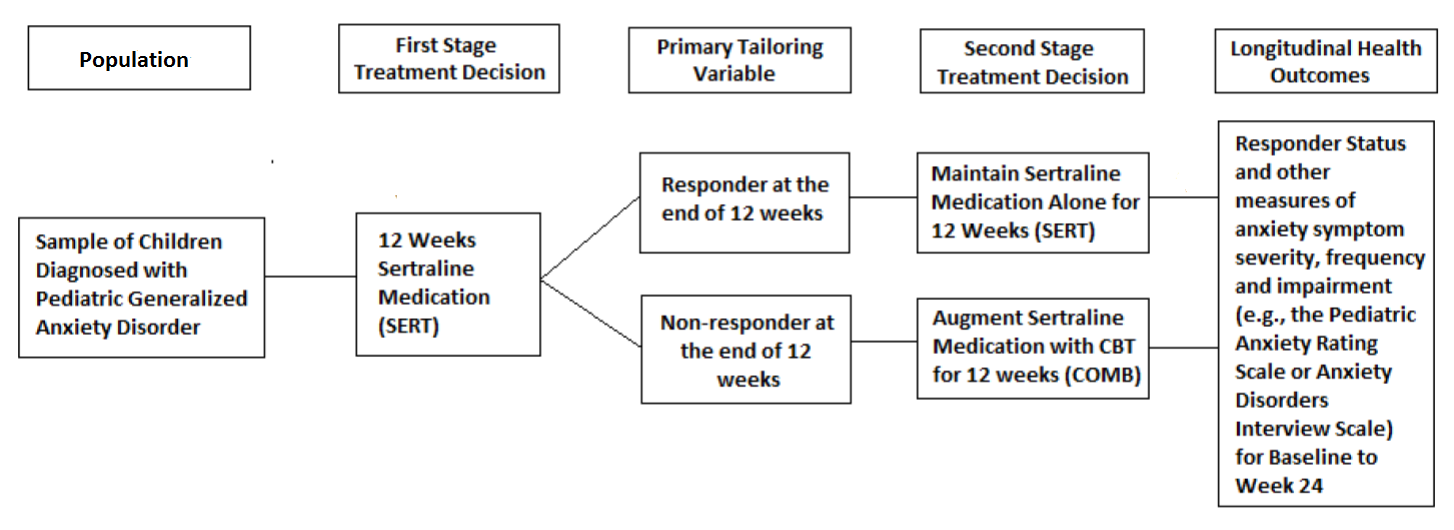
\includegraphics[scale=0.5]{EmbeddedRegime.png}
\end{figure}
\end{frame}

%Another example of using \only for changing the bolding/coloring effects of certain words
\begin{frame}
\frametitle{Addressing the Clinical Aim}
``Identify the optimal dosage regimen of SFN supplementation that achieves the best functional outcome {\only<2>{\textbf}{with}} and {\only<1>{\textbf}{without}} additional tailoring variables."
\vfill 
\begin{minipage}[t]{0.45\textwidth}
	\begin{center}
		{\large Outcomes}
	\end{center}
	\begin{itemize}
		\item Tolerance\\
		\item 6-Minute Walking Distance
	\end{itemize}
\end{minipage}\hfill
\begin{minipage}[t]{0.45\textwidth}
	\begin{center}
		{\large Covariates}
	\end{center}
	\begin{itemize}
		\item SFN Supplementation \\
		\item Dosing \\
		\item Diabetic Status\\
		\item {\only<1>{\textcolor{gray}}{Demographics}} \\
		\item {\only<1>{\textcolor{gray}}{Blood Work}} \\
		\item \textcolor{gray}{Biomarkers}
	\end{itemize}
\end{minipage}
\end{frame}


%%%%%%%%%%%%%%%%%%%%%%%%%%%%%%%%%%%%%%%%%%%%%%%%%%%%%%%%%%%%%%%%%%%%%%%
\section{DNA Damage Repair Subtyping}

\begin{frame}
 \frametitle{DNA Damage Repair (DDR) Motivation}
 \begin{itemize}
	\item Given that Platinum-based chemotherapies act by damaging DNA, it is assumed that tumor cells that have better repair efficiencies.
 \end{itemize}
\end{frame}

\begin{frame}
 \frametitle{Data}
 \begin{itemize}
    \item There are RNA-Seq samples for 376 cases in the available data for the TCGA-OV project. We will restrict the sample to only those with clinical data available.
	  \item The DNA Damage Response (DDR) gene set was retrieved from the Gene Ontology Consortium. It contains 830 genes of which 808 appear in the TCGA samples.
	 \item Conclusion, Summary, Limitations, Future Work
 \end{itemize}
\end{frame}
%
\begin{frame}
 \frametitle{Preprocessing Considerations}
 \begin{itemize}
	\item Dimensionality Reduction: Distance measures in high-dimensional spaces. 
	\item Normalization - Variance Stabilizing Transformation (DESeq2)
	Assume that the number of reads in sample $j$ that are assigned to gene $i$ can be modeled by a negative binomial (NB) distribution,

$K_{ij} \sim NB(\mu_{ij}, \sigma_{ij}^2)$

\item Low counts
 \end{itemize}
\end{frame}

%%%%%%%%%%%%%%%%%%%%%%%%%%%%%%%%%%%%%%%%%%%%%%%%%%%%%%%%%%%%%%%%%%%%%%%


%%%%%%%%%%%%%%%%%%%%%%%%%%%%%%%%%%%%%%%%%%%%%%%%%%%%%%%%%%%%%%%%%%%%%%%
\section{Discussion}
\begin{frame}
\frametitle{Discussion}
\begin{itemize}
	\item Conclusion, Summary, Limitations, Future Work
\end{itemize}

\end{frame}


%%%%%%%%%%%%%%%%%%%%%%%%%%%%%%%%%%%%%%%%%%%%%%%%%%%%%%%%%%%%%%%%%%%%%%%
%Use \backupbegin and \backupend to prevent numbering your appendix slides
\backupbegin

\begin{frame}
 \frametitle{References}
 	\Fontvi
	\begin{enumerate}
		\item Almirall, D., Compton, S. N., Gunlicks-Stoessel, M., Duan, N., and Murphy, S. A. (2012). ``Designing a Pilot Sequential Multiple Assignment Randomized Trial for Developing an Adaptive Treatment Strategy". In: \textit{Statistics in Medicine} 31.17, pp. 1887--1902.
		\item Bien, J., Taylor, J., and Tibshirani, R. (2013). ``A LASSO for Hierarchical Interactions". In: \textit{Annals of Statistics} 41.3, p. 1111.
		\item Kosorok, M. R., Chen, J., Chaudhari, M., Choudhury, A., Cui, Y., Jiang, X., Lawson, M., Luckett, D., Nguyen, C., Pokaprakarn, T., and Laber, E. (2016). ``Design and Sample Size for SMART Studies". IMPACT Symposium. Cary, NC.
		\item Murphy, S. A. (2005). ``An Experimental Design for the Development of Adaptive Treatment Strategies". In: \textit{Statistics in Medicine} 24.10, pp. 1455--1481.
		\item Rich, B., Moodie, E. E., and Stephens, D. A. (2014). ``Simulating Sequential Multiple Assignment Randomized Trials to Generate Optimal Personalized Warfarin Dosing Strategies". In: \textit{Clinical Trials} 11.4, pp. 435--444.
		\item Zhao, Y. (2015) ``Reinforcement Learning Applications in Clinical Trials". In: \textit{Adaptive Treatment Strategies in Practice: Planning Trials and Analyzing Data for Personalized Medicine}. Ed. by M. Kosorok and E. Moodie. SIAM. Chap. 17.
	\end{enumerate}
\end{frame}

\backupend

\end{document}